\documentclass[letterpaper,11pt]{article}
\usepackage[spanish]{babel}
\usepackage[utf8]{inputenc}
\usepackage{graphicx}
\usepackage{amsfonts,amsmath,amssymb,float, amsthm,mathrsfs}  
\usepackage[right=4.5cm,left=2cm,top=3cm,bottom=3cm,headsep= 0.7cm,footskip=0.5cm]{geometry}
\usepackage{enumerate}
\usepackage{wrapfig} 
\usepackage[rflt]{floatflt} 
\usepackage{framed}
%\usepackage[most]{tcolorbox}
\usepackage[dvipsnames]{xcolor}
\colorlet{shadecolor}{green!20}
\setlength\FrameSep{0.5ex}
\usepackage{thmtools}
\usepackage{esint}
\usepackage{cancel}
\usepackage{listings} 
\usepackage{pstricks, caption}
\usepackage[colorlinks]{hyperref}
\usepackage{csquotes}
\usepackage{fullpage}
\usepackage{enumitem}
\usepackage{etoolbox}
\usepackage{tikz}
\usepackage{tikz-3dplot}
\tdplotsetmaincoords{80}{70}
\usetikzlibrary{decorations.markings}
\usetikzlibrary{arrows,babel}
\usepackage[font=small]{caption}
\usepackage{scalerel} %\scaleto{text}{size}
\usepackage{subfigure}
\usepackage{fancyhdr}
\usepackage{comment}
\usepackage{marginnote}
\usepackage{tensor}
\usepackage{cleveref}
\newcommand{\dbar}{\mathchar'26\mkern-12mu d}
\renewcommand*{\marginnotevadjust}{-0.1cm}
\renewcommand*{\marginfont}{\footnotesize}
\setlength{\headheight}{15pt}
\addtolength{\topmargin}{-14.49998pt}
\setlength{\headsep}{15pt}
\setlength{\footskip}{14.49998pt}
\decimalpoint
\newcommand{\grad}{^\circ}
\newlength{\drop}
\DeclareMathOperator{\sign}{sgn}
\DeclareMathOperator{\Log}{Log}
\providecommand{\norm}[1]{\lVert#1\rVert}

\let\cancelorigcolor\CancelColor% Just for conveniency...

\newcommand{\CancelTo}[3][]{%
  \ifblank{#1}{}{%
    \renewcommand{\CancelColor}{#1}%
  }
  \cancelto{#2}{#3}% 
}


\begin{document}

\pagestyle{plain}

\begin{flushleft}\vspace{-2cm}
Departamento de Física \\
Facultad de Cs. Físicas y Matemáticas\\
Universidad de Concepción
\end{flushleft}

\begin{flushright}\vspace{-1.5cm}
\textbf{Tópicos en Relatividad General} 
\end{flushright}



\rule{\linewidth}{0.1mm}

\begin{center}
\textbf{\LARGE Semana 8}
\end{center}

\begin{flushleft}
\textbf{Nombre:} Alejandro Saavedra San Martín. \\
\textbf{Profesor:} Guillermo Rubilar Alegría.
\end{flushleft}

\section*{Tiempo de Vuelo (Efecto Shapiro)}

Estudiaremos la predicción de la teoría de Eisntein de la gravitación en lo que respecta al tiempo de vuelo de señales luminosas en la métrica de Schwarzschild. Por ejemplo, consideremos que enviamos una señal luminosa desde la Tierra hasta Venus, luego la señal vuelve a la Tierra, durante todo el proceso consideraremos que ambos planetas están quietos, ver figura \ref{fig:Efecto-Shapiro} para una descripción pictórica de la situación física.

\begin{figure}[H]
    \centering
    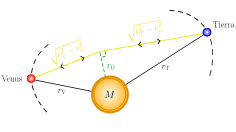
\includegraphics[scale = 0.5]{Fig-Tiempo-Vuelo-1}
    \caption{Esquema de la situación física.}
    \label{fig:Efecto-Shapiro}
\end{figure}

Para obtener información del tiempo de vuelo de una señal luminosa debemos analizar cómo cambia la coordenada radial temporal $t$ a lo largo de la línea de mundo del rayo de luz. Para ello, usaremos la cantidad conservada en una geodésica tipo luz encontrada en el documento de la semana 5:
\begin{equation}
\frac{r^2}{\left(1 - \frac{2m}{r} \right)} \frac{d\varphi}{dt} = \frac{c}{\alpha}.
\end{equation}

Si suponemos $r = r(t)$, por regla de la cadena,
\begin{equation}
\frac{dr}{dt} = \frac{dr}{d\varphi} \frac{d\varphi}{dt} = r' \frac{c}{\alpha} \left( 1 - \frac{2m}{r}\right) \frac{1}{r^2}, \label{eq:Shapiro-1}
\end{equation}
donde $r' = dr/d\varphi$. Del mismo documento de la semana 5 probamos que la dinámica radial está contenida en la siguiente ecuación diferencial a primer orden en $r$:
\begin{equation}
r'^2 + r^2 -2mr -\alpha^2 r^4 = 0. \label{eq:Shapiro-1.5}
\end{equation}

Despejando $r'$, tenemos que
\begin{equation}
r' = \pm \sqrt{-r^2 + 2mr + \alpha^2r^4}. \label{eq:Shapiro-2}
\end{equation}

Reemplazando \eqref{eq:Shapiro-2} en \eqref{eq:Shapiro-1}:
\begin{align}
\frac{dr}{dt} &= \pm \sqrt{-r^2 + 2mr + \alpha^2r^4} \frac{c}{\alpha} \left(1 - \frac{2m}{r} \right) \frac{1}{r^2} \\
\frac{1}{c} \frac{dr}{dt} &= \pm \frac{1}{\alpha} \left( 1 - \frac{2m}{r}\right)\sqrt{\alpha^2 + \frac{2m}{r^3} - \frac{1}{r^2}}.
\end{align}

Si definimos
\begin{equation}
I(r) := \frac{1}{\alpha} \left(1 - \frac{2m}{r} \right) \sqrt{\alpha^2 + \frac{2m}{r^3} - \frac{1}{r^2}}, \label{eq:Shapiro-3}
\end{equation}
hemos encontrado que
\begin{equation}
\frac{1}{c} \frac{dr}{dt} = \pm I(r).\label{eq:Shapiro-4}
\end{equation}

El fotón se mueve desde la Tierra en un punto con coordenada $(ct_{\text{T}},r_{\text{T}},\pi/2,\varphi_{\text{T}})$ hacia el centro de fuerzas, hasta el punto $(ct_0,r_0,\pi/2,\varphi_0)$ de máximo acercamiento, ver figura \ref{fig:Efecto-Shapiro}. En este primer tramo $dr/dt < 0$ y entonces, al integrar \eqref{eq:Shapiro-4}, tenemos que
\begin{align}
\frac{1}{c} \frac{dr}{dt} &= -I(r) \\
c\,dt &= -\frac{dr}{I(r)} \\
\int_{t_{\text{T}}}^{t_0} dt &= - \int_{r_{\text{T}}}^{r_0} \frac{dr}{I(r)} \\
c(t_0 - t_{\text{T}}) &= - \int_{r_{\text{T}}}^{r_0} \frac{dr}{I(r)}. \label{eq:Shapiro-5}
\end{align}

Para el segundo tramo (punto de máximo acercamiento a Venus), desde $(ct_0,r_0,\pi/2,\varphi_0)$ hasta $(ct_{\text{V}}, r_{\text{V}},\pi/2,\varphi_{\text{V}})$, ver figura \ref{fig:Efecto-Shapiro}, tenemos que $dr/dt > 0$ y entonces
\begin{equation}
c(t_{\text{V}} - t_0) = \int_{r_0}^{r_{\text{V}}} \frac{dr}{I(r)}. \label{eq:Shapiro-6}
\end{equation} 

El intervalo total de coordenada temporal en el proceso de vuelo (``de ida") es entonces dado por $t_{\text{V}} - t_{\text{T}}$. Sumando \eqref{eq:Shapiro-5} y \eqref{eq:Shapiro-6} obtenemos
\begin{align}
c(t_{\text{V}} - t_{\text{T}}) &= \int_{r_0}^{r_{\text{V}}} \frac{dr}{I(r)} - \int_{r_{\text{T}}}^{r_0} \frac{dr}{I(r)} \nonumber \\
&= \int_{r_0}^{r_{\text{V}}} \frac{dr}{I(r)} - \int_{r_0}^{r_{\text{T}}} \frac{dr}{I(r)}  \label{eq:Shapiro-6.5}
\end{align}

Para evaluar esta expresión es necesario escribir $\alpha$ en términos de $r_0 = r_{\text{min}}$, la coordenada radial mínima al centro de fuerzas sobre la trayectoria del fotón. Esta coordenada mínima se encuentra con la solución perturbada para una geodésica tipo luz:
\begin{equation}
u(\varphi) = \frac{1}{D} \left[ \sin(\varphi-\varphi_0) + \frac{m}{D}[1 + \cos^2(\varphi-\varphi_0)]\right] + \mathcal{O}(\epsilon^2),
\end{equation}
donde $u = 1/r$. Si derivamos con respecto a $\varphi$:
\begin{align}
u'(\varphi) &= \frac{1}{D} \cos(\varphi - \varphi_0) - \frac{2m}{D^2} \cos(\varphi-\varphi_0) \sin(\varphi-\varphi_0) \nonumber \\
&= \frac{1}{D}\cos(\varphi - \varphi_0) \left[ 1 - \frac{2m}{D} \sin(\varphi_0 - \varphi_0) \right].
\end{align}

Como $D \gg m$, es imposible que el segundo factor se anule. Por tanto, los puntos críticos de $u(\varphi)$ (en el esquema perturbativo) son los $\varphi$ tales que 
\begin{equation}
\cos(\varphi - \varphi_0) = 0 \Leftrightarrow \varphi = \varphi_0 + \frac{\pi}{2} + k\pi, \quad k \in \mathbb{Z}. 
\end{equation} 

Si tomamos $k = 0$, comprobemos que para $\varphi = \varphi_0 + \pi/2$ se obtiene un máximo de $u$ (lo que equivale a un mínimo de $r$).  Calculemos la segunda derivada:
\begin{equation}
u''(\varphi) = - \frac{1}{D} \sin(\varphi - \varphi_0) - \frac{2m}{D^2} \left[-\sin^2(\varphi - \varphi_0) + \cos^2(\varphi-\varphi_0)\right].
\end{equation}

Evaluando en $\varphi = \varphi_0 + \pi/2$, obtenemos que
\begin{equation}
u''\left(\varphi_0 + \frac{\pi}{2}\right) = - \frac{1}{D} + \frac{2m}{D^2} = \frac{2m -D}{D^2} < 0,
\end{equation}
por el criterio de la segunda derivada para puntos críticos, en  $\varphi = \varphi_0 + \pi/2$ se alcanza un máximo de $u$ igual a
\begin{equation}
u_{\text{máx}} = u\left(\varphi_0 + \frac{\pi}{2}\right) = \frac{1}{D} + \frac{m}{D^2} = \frac{D + m}{D^2}.
\end{equation}

Por definición, $u = 1/r$. Así,
\begin{equation}
r_{\text{mín}} = \frac{1}{u_{\text{máx}}} = \frac{D^2}{D+m} =  \frac{D}{1 + \frac{m}{D}} = D \left( 1 - \frac{m}{D} \right) + \mathcal{O}\left( \frac{m^2}{D^2}\right).
\end{equation}

Si $\epsilon = 3m/D$, entonces
\begin{equation}
r_0 = r_{\text{mín}} = D\left(1 - \frac{m}{D}\right) + \mathcal{O}(\epsilon^2).
\end{equation}

Evaluando \eqref{eq:Shapiro-1.5} para $r = r_0$, tenemos que $r' = 0$.  Luego,
\begin{align}
r_0^2 -2mr_0 - \alpha^2 r_0^4 &= 0 \\
\alpha^2 r_0^4 &= r_0^2 - 2mr_0 \\
\alpha^2 &= \frac{1}{r_0^2} \left(1 - \frac{2m}{r_0} \right) \\
\alpha &= \frac{1}{r_0} \sqrt{1 - \frac{2m}{r_0}}.
\end{align}

Expandiendo en serie de Taylor la raíz para $r_0 \gg m$:
\begin{equation}
\alpha = \frac{1}{r_0}\left(1 - \frac{m}{r_0}\right) + \mathcal{O}\left(\epsilon\right),
\end{equation}
donde hemos redefinido $\epsilon := 3m/r_0$.

Con esto, podemos expresar la función $I(r)$ como 
\begin{align}
I(r) &= \frac{1}{\alpha}\left( 1 - \frac{2m}{r}\right)\sqrt{\alpha^2 + \frac{2m}{r^3} - \frac{1}{r^2}} \nonumber\\
&= r_0 \textcolor{red}{\left(\frac{1}{1-\frac{m}{r_0}}\right)} \left(1 - \frac{2m}{r} \right) \sqrt{\frac{1}{r_0^2}\left( 1 - \frac{2m}{r_0}\right) + \frac{2m}{r^3} - \frac{1}{r^2}} \nonumber \\
&= r_0 \textcolor{red}{\left(1 + \frac{m}{r_0} + \mathcal{O}(\epsilon^2) \right)} \left(1 - \frac{2m}{r}\right) \sqrt{\frac{1}{r_0^2} - \frac{2m}{r_0^3} + \frac{2m}{r^3} - \frac{1}{r^2}} \nonumber\\
&= \left( 1 + \frac{m}{r_0} \right) \left( 1 - \frac{2m}{r}\right) \sqrt{1 - \frac{2m}{r_0} + 2m \frac{r_0^2}{r^3} - \frac{r_0^2}{r^2}} + \mathcal{O}(\epsilon^2) \nonumber\\
&= \left( 1 - \frac{2m}{r} + \frac{m}{r_0}\right) \sqrt{1 - \frac{r_0^2}{r^2} - \frac{2m}{r_0}\left( 1 - \frac{r_0^3}{r^3}\right)} + \mathcal{O}(\epsilon^2). \label{eq:Shapiro-7}
\end{align}

De la última línea, si consideramos la raíz como una función de $m/r_0$ y expandimos en serie de Taylor en torno a $m/r_0$, tenemos que
\begin{equation}
\sqrt{1 - \frac{r_0^2}{r^2} - \frac{2m}{r_0}\left( 1 - \frac{r_0^3}{r^3}\right)} =   \sqrt{1 - \frac{r_0^2}{r^2}} - \frac{2}{2\sqrt{1 - \frac{r_0^2}{r^2}}}  \left(1 - \frac{r_0^3}{r^3}\right ) \frac{m}{r_0} + \mathcal{O}(\epsilon^2).\label{eq:Shapiro-8}
\end{equation} 

Reemplazando \eqref{eq:Shapiro-8} en \eqref{eq:Shapiro-7}:
\begingroup
\allowdisplaybreaks
\begin{align}
I(r) &=  \left( 1 - \frac{2m}{r} + \frac{m}{r_0}\right) \left[ \sqrt{1 - \frac{r_0^2}{r^2}} - \frac{1}{\sqrt{1 - \frac{r_0^2}{r^2}}}  \left(1 - \frac{r_0^3}{r^3}\right ) \frac{m}{r_0}\right] + \mathcal{O}(\epsilon^2) \nonumber \\
&= \left( 1 - \frac{2m}{r} + \frac{m}{r_0}\right) \sqrt{1 - \frac{
r_0^2}{r^2}} \left[1 - \frac{m}{r_0} \frac{1 - \frac{r_0^3}{r^3}}{1 - \frac{r_0^2}{r^2}} \right] + \mathcal{O}(\epsilon^2) \nonumber\\
&= \left( 1 - \frac{2m}{r} + \frac{m}{r_0}\right) \sqrt{1 - \frac{
r_0^2}{r^2}} \left[1 - \frac{m}{r_0} \frac{\left(1 - \frac{r_0}{r}\right)\left(1 + \frac{r_0}{r} + \frac{r_0^2}{r^2}\right)}{\left(1 - \frac{r_0}{r}\right)\left(1 + \frac{r_0}{r}\right)} \right] + \mathcal{O}(\epsilon^2) \nonumber \\
&= \left( 1 - \frac{2m}{r} + \frac{m}{r_0}\right) \sqrt{1 - \frac{
r_0^2}{r^2}} \left[1 - \frac{m}{r_0} \frac{\left(1 + \frac{r_0}{r} + \frac{r_0^2}{r^2}\right)}{\left(1 + \frac{r_0}{r}\right)} \right] + \mathcal{O}(\epsilon^2) \nonumber  \\
&=  \sqrt{1 - \frac{r_0^2}{r^2}} \left[ 1 - \frac{m}{r_0} \frac{\left(1 + \frac{r_0}{r} + \frac{r_0^2}{r^2}\right)}{\left(1 + \frac{r_0}{r}\right)} - \frac{2m}{r} + \CancelTo[\color{red}]{\approx 0}{\frac{2m^2}{rr_0} \frac{\left(1 + \frac{r_0}{r} + \frac{r_0^2}{r^2}\right)}{\left(1 + \frac{r_0}{r}\right)}} + \frac{m}{r_0} \right. \nonumber \\
&\qquad \left. - \CancelTo[\color{red}]{\approx 0}{\frac{m^2}{r_0^2} \frac{\left(1 + \frac{r_0}{r} + \frac{r_0^2}{r^2}\right)}{\left(1 + \frac{r_0}{r}\right)}}  \right] + \mathcal{O}(\epsilon^2) \nonumber \\
&= \sqrt{1 - \frac{r_0^2}{r^2}} \left[1 - \frac{m}{r_0}\left(1 + \frac{r_0^2}{r(r+r_0)} \right) - \frac{2m}{r} + \frac{m}{r_0} \right] + \mathcal{O}(\epsilon^2) \nonumber \\
&= \sqrt{1 - \frac{r_0^2}{r^2}} \left[1 - \frac{mr_0}{r(r + r_0)} - \frac{2m}{r} \right] + \mathcal{O}(\epsilon^2).
\end{align}
\endgroup

De esta forma, obtenemos
\begin{align}
\frac{1}{I(r)} &= \frac{1}{\sqrt{1 - \frac{r_0^2}{r^2}}} \frac{1}{1 - \frac{mr_0}{r(r + r_0)} - \frac{2m}{r}} \nonumber\\
&= \frac{1}{\sqrt{1 - \frac{r_0^2}{r^2}}} \left(1 + \frac{mr_0}{r(r+r_0)} + \frac{2m}{r}\right) + \mathcal{O}(\epsilon^2).
\end{align}

Entonces, integrando con respecto a $r$, encontramos que
\begin{align}
\int \frac{dr}{I(r)} &= \int \frac{1}{\sqrt{1 - \frac{r_0^2}{r^2}}} \left[1 + \frac{mr_0}{r(r + r_0)} + \frac{2m}{r}\right] \,dr + \mathcal{O}(\epsilon^2) \nonumber\\
&= \sqrt{r^2 - r_0^2} + 2m \ln\left(r + \sqrt{r^2 - r_0^2}\right) + m \sqrt{\frac{r-r_0}{r + r_0}} + \mathcal{O}(\epsilon^2).
\end{align}

El cálculo explícito de la integral se encuentra en el siguiente \href{https://github.com/AleSaa66/Topicos-RG/blob/main/Semana%208/Semana-8.ipynb}{notebook}.

Con este resultado podemos evaluar el intervalo (de coordenada temporal) $(\Delta t)_{\text{ir}}$ de ``ida y regreso" que, de acuerdo a \eqref{eq:Shapiro-6.5}, es entonces dado por
\begin{align}
\frac{c}{2} (\Delta t)_{\text{ir}} &= \int_{r_0}^{r_{\text{V}}} \frac{dr}{I(r)} + \int_{r_0}^{r_{\text{T}}} \frac{dr}{I(r)} \nonumber \\
&= \left[\sqrt{r^2 - r_0^2} + 2m \ln\left(r+ \sqrt{r^2-r_0^2}\right) + m \sqrt{\frac{r-r_0}{r+r_0}} \right]_{r_0}^{r_{\text{V}}} \nonumber\\
& \quad + \left[\sqrt{r^2 - r_0^2} + 2m \ln\left(r+ \sqrt{r^2-r_0^2}\right) + m \sqrt{\frac{r-r_0}{r+r_0}} \right]_{r_0}^{r_{\text{T}}} \nonumber\\
&= \sqrt{r_{\text{V}}^2 - r_0^2} + 2m\ln\left(r_{\text{V}} + \sqrt{r_{\text{V}}^2 - r_0^2}\right) + m \sqrt{\frac{r_{\text{V}} - r_0}{r_{\text{V}} + r_0}} - 2m \ln(r_0) \nonumber\\
&\quad + \sqrt{r_{\text{T}}^2 - r_0^2} + 2m \ln\left(r_{\text{T}} + \sqrt{r_{\text{T}}^2 - r_0^2}\right) +  m \sqrt{\frac{r_{\text{T}} - r_0}{r_{\text{T}} + r_0}} - 2m \ln(r_0)\nonumber\\
&= \sqrt{r_{\text{V}}^2 - r_0^2} + \sqrt{r_{\text{T}}^2 - r_0^2} + 2m \ln\left[\left(r_{\text{V}} + \sqrt{r_{\text{V}}^2 - r_0^2}\right)\left(r_{\text{T}} + \sqrt{r_{\text{T}}^2 - r_0^2}\right)\right] - 2m \ln(r_0^2) \nonumber\\
&\quad + m \left(\sqrt{\frac{r_{\text{V}} - r_0}{r_{\text{V}} + r_0}} + \sqrt{\frac{r_{\text{T}} - r_0}{r_{\text{T}} + r_0}}\right) + \mathcal{O}(\epsilon^2) \nonumber\\
&= \sqrt{r_{\text{V}}^2 - r_0^2} + \sqrt{r_{\text{T}}^2 - r_0^2} + 2m \ln\left[\frac{\left(r_{\text{V}} + \sqrt{r_{\text{V}}^2 - r_0^2}\right)\left(r_{\text{T}} + \sqrt{r_{\text{T}}^2 - r_0^2}\right)}{r_0^2} \right] \nonumber\\
&\quad  + m \left(\sqrt{\frac{r_{\text{V}} - r_0}{r_{\text{V}} + r_0}} + \sqrt{\frac{r_{\text{T}} - r_0}{r_{\text{T}} + r_0}}\right) + \mathcal{O}(\epsilon^2).
\end{align}

En el caso que $r_0 = R_{\odot} \ll r_{\text{V}}, r_{\text{T}}$ (``conjunción superior") el efecto es máximo:
\begin{align}
\frac{c}{2} (\Delta t)_{\text{ir}} &\approx 2 \left[ r_{\text{V}} + r_{\text{T}}  +2m \ln\left( \frac{(r_{\text{V}} + r_{\text{V}})(r_{\text{T}} + r_{\text{T}})}{R_{\odot}^2}\right) + m \left( \sqrt{\frac{1 - \frac{r_0}{r_{\text{V}}}}{1 + \frac{r_0}{r_{\text{V}}}}} + \sqrt{\frac{1 - \frac{r_0}{r_{\text{T}}}}{1 + \frac{r_0}{r_{\text{T}}}}} \right)\right] \nonumber\\
&\approx 2 \left[ r_{\text{V}} + r_{\text{T}} + 2m \ln\left(\frac{4r_{\text{V}} r_{\text{T}}}{R_{\odot}^2}\right)+ m \left( \sqrt{\left(1 - \frac{r_0}{r_{\text{V}}}\right)\left(1 + \frac{r_0}{r_{\text{V}}}\right)} + \sqrt{\left(1 - \frac{r_0}{r_{\text{T}}}\right)\left(1 + \frac{r_0}{r_{\text{T}}}\right)}\right) \right] \nonumber\\
&\approx  2 \left[ r_{\text{V}} + r_{\text{T}} + 2m \ln\left(\frac{4r_{\text{V}} r_{\text{T}}}{R_{\odot}^2}\right)+ m(1 + 1) \right] \nonumber\\
&= 2 \left[(r_{\text{V}} + r_{\text{T}}) + 2m \left(1 + \ln\left[\frac{4r_{\text{V}} r_{\text{T}}}{R_{\odot}^2}\right]\right)\right]. \label{eq:Shapiro-9}
\end{align}

\end{document}
